\documentclass[tikz,border=7pt]{standalone}
\usepackage{amsmath,amssymb}
\usepackage[scaled]{helvet}
\renewcommand{\familydefault}{\sfdefault}
\usetikzlibrary{arrows.meta,backgrounds,calc,fit,positioning,shapes.geometric}
\definecolor{bpink}{HTML}{172033}
\definecolor{bpblue}{HTML}{2A78D6}
\definecolor{bporange}{HTML}{E56A32}
\definecolor{bpgreen}{HTML}{168A65}
\definecolor{bppurple}{HTML}{7A5CC7}
\definecolor{bpred}{HTML}{C94A4A}
\definecolor{bpmuted}{HTML}{667085}
\definecolor{bpgrid}{HTML}{D8DEE8}
\definecolor{bpsurface}{HTML}{F8FAFC}
\tikzset{
  var/.style={circle,draw=bpblue,fill=bpblue!10,line width=.9pt,minimum size=8mm,font=\small\bfseries,text=bpink},
  factor/.style={rectangle,rounded corners=1.5pt,draw=bporange,fill=bporange!14,line width=.9pt,minimum size=6.8mm,font=\small\bfseries,text=bpink},
  constraint/.style={rectangle,rounded corners=1.5pt,draw=bpred,fill=bpred!12,line width=.9pt,minimum size=6.8mm,font=\small\bfseries,text=bpink},
  edge/.style={draw=bpmuted!75,line width=.9pt},
  msgvf/.style={-{Latex[length=2.2mm]},draw=bpblue,line width=1.35pt},
  msgfv/.style={-{Latex[length=2.2mm]},draw=bporange,line width=1.35pt},
  label/.style={font=\scriptsize,text=bpmuted,align=center},
  title/.style={font=\bfseries\large,text=bpink},
  card/.style={draw=bpgrid,fill=bpsurface,rounded corners=7pt,line width=.7pt},
}

\begin{document}
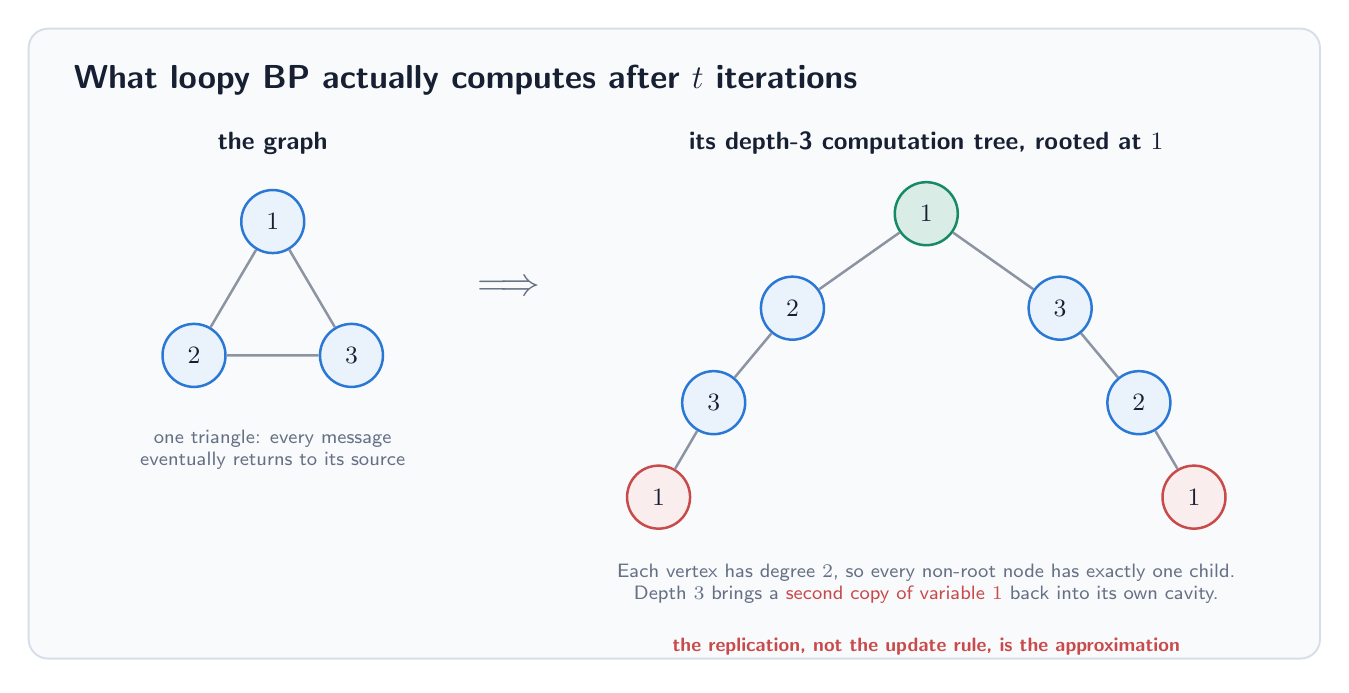
\begin{tikzpicture}[font=\sffamily]
  \node[card,minimum width=16.4cm,minimum height=8.0cm] at (7.4,2.7) {};
  \node[title,anchor=west] at (-.35,6.05) {What loopy BP actually computes after $t$ iterations};

  \node[text=bpink,font=\small\bfseries] at (2.3,5.25) {the graph};
  \node[var] (a1) at (2.3,4.25) {$1$};
  \node[var] (a2) at (1.3,2.55) {$2$};
  \node[var] (a3) at (3.3,2.55) {$3$};
  \draw[edge] (a1)--(a2)--(a3)--(a1);
  \node[label,align=center] at (2.3,1.35) {one triangle: every message\\eventually returns to its source};

  \node[text=bpmuted,font=\Large] at (5.3,3.4) {$\Longrightarrow$};

  \node[text=bpink,font=\small\bfseries] at (10.6,5.25) {its depth-3 computation tree, rooted at $1$};
  \node[var,draw=bpgreen,fill=bpgreen!16] (r) at (10.6,4.35) {$1$};
  \node[var] (l1) at (8.9,3.15) {$2$};
  \node[var] (l2) at (7.9,1.95) {$3$};
  \node[var,draw=bpred,fill=bpred!10] (l3) at (7.2,.75) {$1$};
  \node[var] (r1) at (12.3,3.15) {$3$};
  \node[var] (r2) at (13.3,1.95) {$2$};
  \node[var,draw=bpred,fill=bpred!10] (r3) at (14.0,.75) {$1$};
  \draw[edge] (r)--(l1)--(l2)--(l3);
  \draw[edge] (r)--(r1)--(r2)--(r3);
  \node[label,align=center] at (10.6,-.35) {Each vertex has degree $2$, so every non-root node has exactly one child.\\Depth $3$ brings a \textcolor{bpred}{second copy of variable $1$} back into its own cavity.};
  \node[text=bpred,font=\scriptsize\bfseries] at (10.6,-1.15) {the replication, not the update rule, is the approximation};
\end{tikzpicture}
\end{document}
